%% Template for ENG 401 reports
%% by Robin Turner
%% Adapted from the IEEE peer review template

%
% note that the "draftcls" or "draftclsnofoot", not "draft", option
% should be used if it is desired that the figures are to be displayed in
% draft mode.

\documentclass[peerreview]{IEEEtran}
\usepackage{cite} % Tidies up citation numbers.
\usepackage{url} % Provides better formatting of URLs.
\usepackage{booktabs} % Allows the use of \toprule, \midrule and \bottomrule in tables for horizontal lines
\usepackage{graphicx}
\graphicspath{.}

\usepackage{subfig}

\usepackage{amsmath}
\usepackage{amsfonts}
\usepackage{amssymb}

\usepackage[T1]{fontenc}
%\usepackage[Polish]{babel}
\usepackage[utf8]{inputenc}

\usepackage{lipsum}




\hyphenation{op-tical net-works semi-conduc-tor} % Corrects some bad hyphenation 



\begin{document}


%\begin{titlepage}
% paper title
% can use linebreaks \\ within to get better formatting as desired
\title{Raport z badania CFD\\ trzech wariantów geometrycznych przekładek}


% author names and affiliations

\author{Lewandowska Natalia \\
Katedra Techniki Cieplnej\\
Politechnika Poznańska\\
}
\date{\today}

% make the title area
\maketitle
\tableofcontents
\listoffigures
\listoftables
%\end{titlepage}

\IEEEpeerreviewmaketitle

\begin{abstract}

\lipsum[1]

\end{abstract}





\section{Wstęp}
This will be a revised version of the introduction in your proposal.

\section{Opis problemu badawczego}
This will be a revised version of the problem definition in your proposal.


\begin{figure}[!h]
\centering
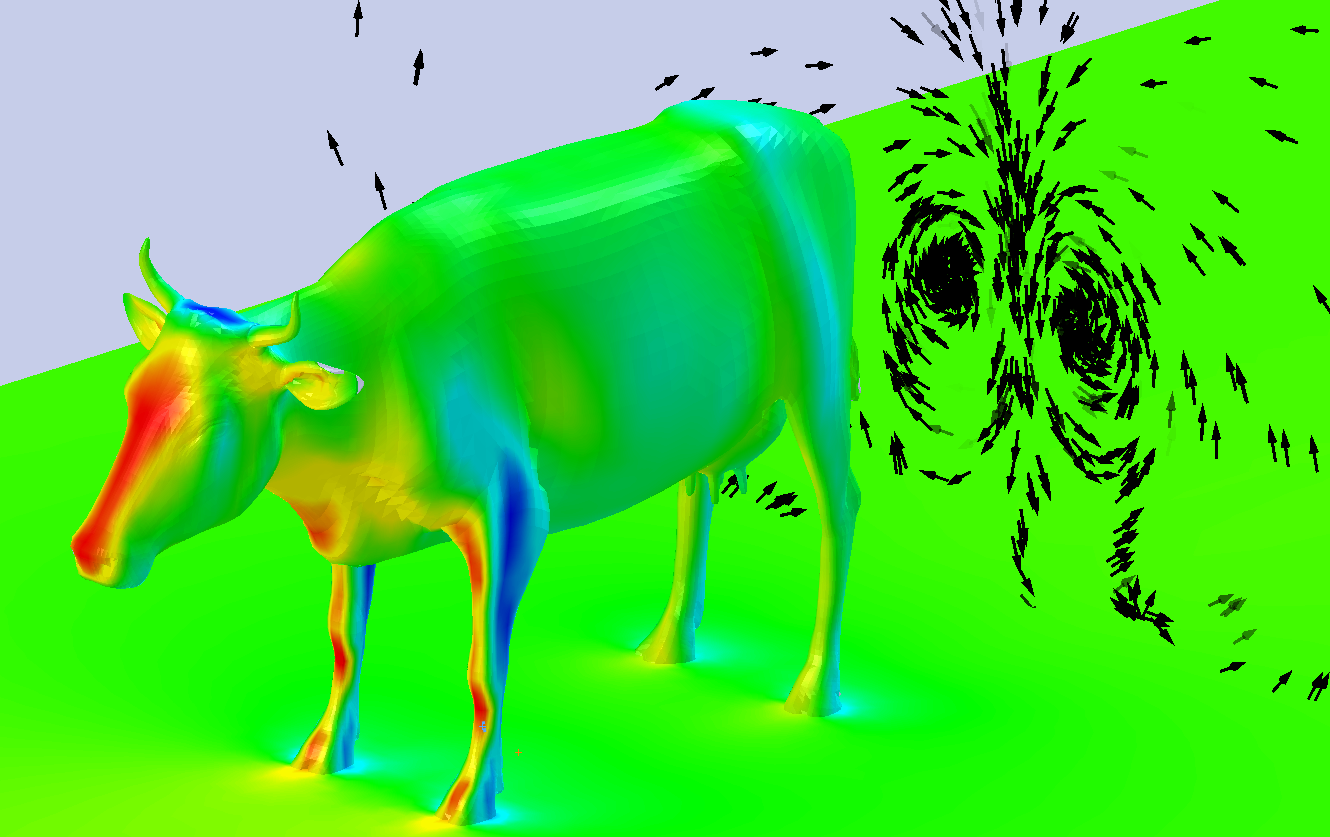
\includegraphics[width=0.8\columnwidth]{placeholder} 
\caption{Simulation Results}
\label{fig_sim}
\end{figure}

% Note that IEEE typically puts floats only at the top, even when this
% results in a large percentage of a column being occupied by floats.

\section{Metodyka badań}
  
\subsection{Założenia projektowe}
nieściśliwość, przepływ laminarny, gładkie ścianki, przeływ jednofazowy --> uzasadnienie: badania miały na celu ukazanie najlepszego pod względem przepływowym wariantu geometrycznego, dlatego poczynione uproszczenia są uzasadnione
\subsection{Warunki brzegowe}
tutaj rysunek przekładki z rozpisanymi warunkami brzegowymi plus każdy opisać: jaka wartość prędkości na wylocie, kierunek, warunek ciśnieniowy na wylocie, no-slip wall  
\subsection{Siatka obliczeniowa}
Screeny siatki, parametry siatki (ortogonalność, skewness, quality determinant?), liczba i typy elementów,
\subsection{Model analityczny, model turbulencji}
równania ciągłosci i pędu, równania dla k-omega SST w ramach cytowania, uzasadnienie wyboru k-omega SST 
\subsection{Parametry solvera numerycznego}
specjalnie wyselekcjonowany schemat numeryczny dedykowany dla nieściśliwych przepływów stancjonarych cieczy newtonowskich, 



\section{Wyniki badań CFD} \label{sec:criteria}

\subsection{Rozkłady prędkości na wlocie, w połowie długości przekładki i na wylocie}
tutaj obrazki przekrojów z CFD, wykresy rozkładu, 

\begin{figure*}
  \centering
  \raisebox{5pt}{\parbox[b]{.1\textwidth}{wariant 1}}%
  \subfloat[][]{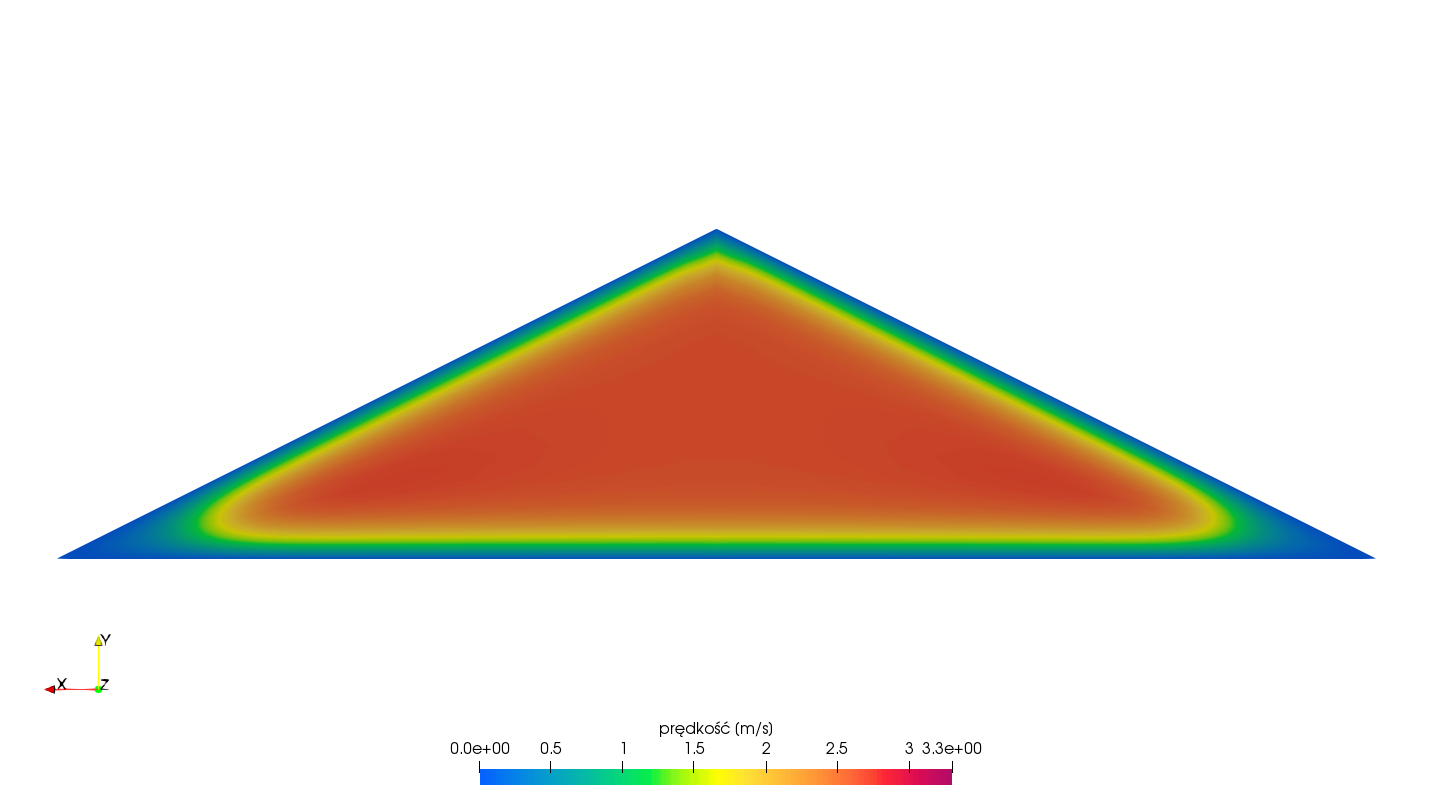
\includegraphics[width=.28\textwidth]{case_01_inlet_velocity}}\hfill
  \subfloat[][]{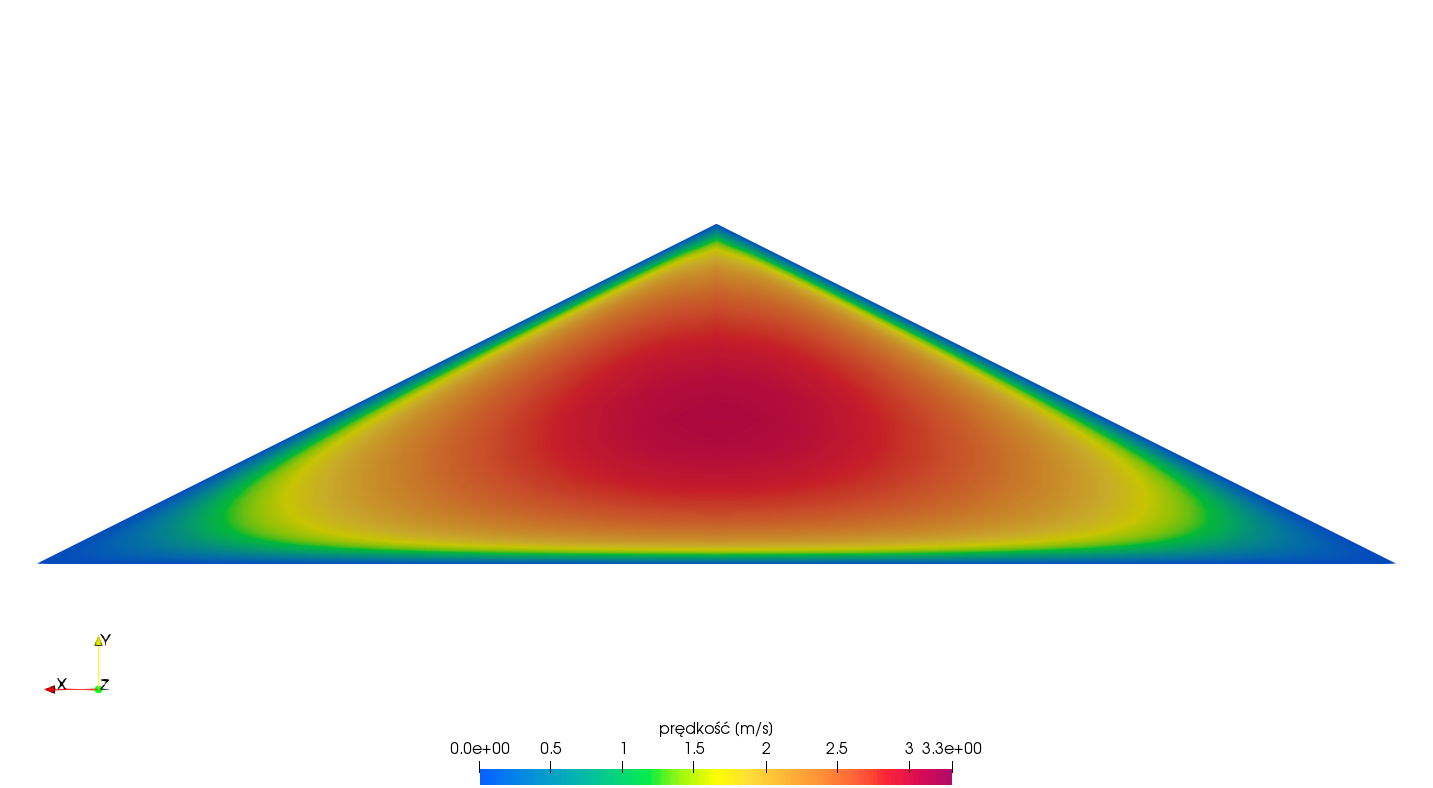
\includegraphics[width=.28\textwidth]{case_01_middle_plane_velocity}}\hfill
  \subfloat[][]{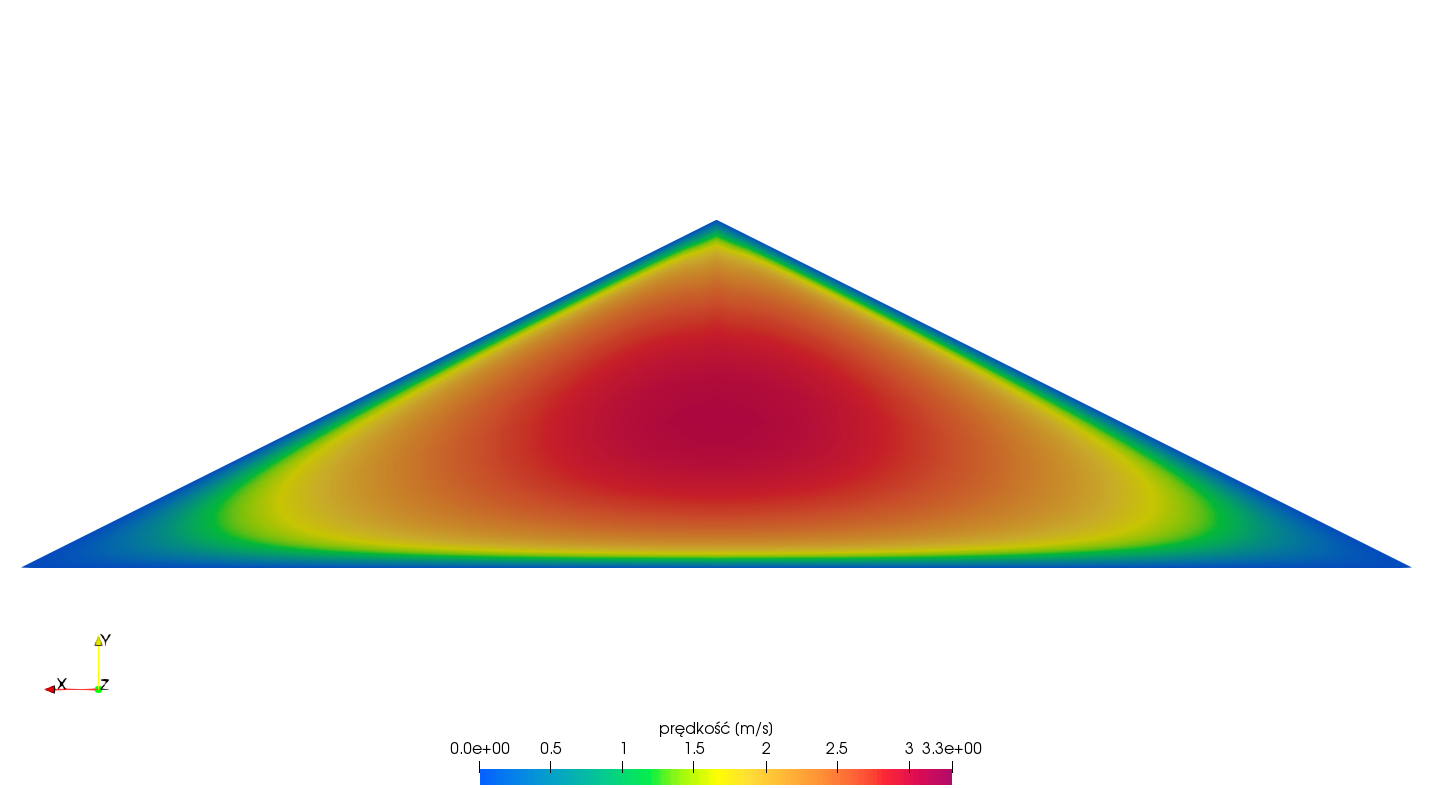
\includegraphics[width=.28\textwidth]{case_01_outlet_velocity}}\par
  \raisebox{5pt}{\parbox[b]{.1\textwidth}{wariant 2}}%
  \subfloat[][]{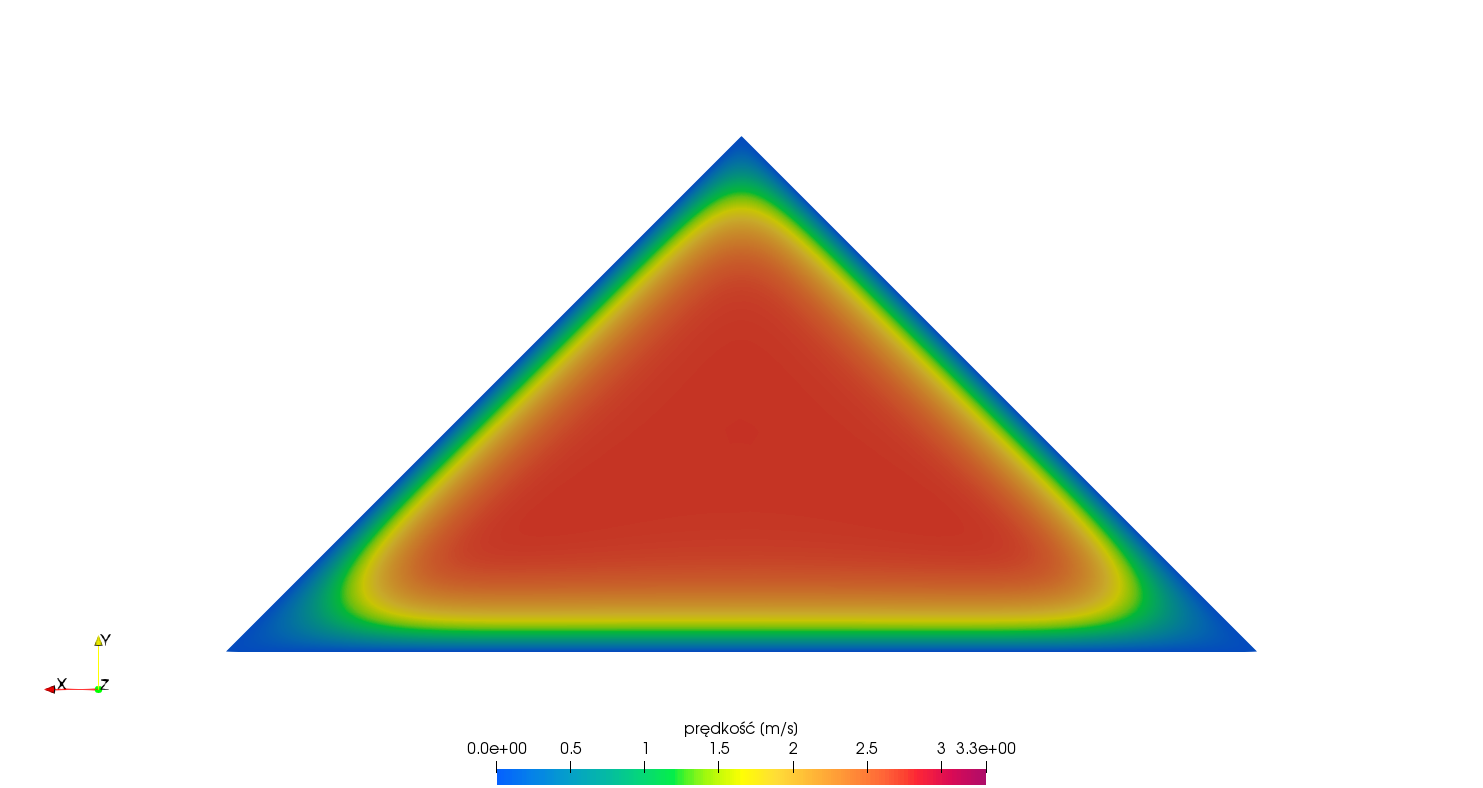
\includegraphics[width=.28\textwidth]{case_02_inlet_velocity}}\hfill
  \subfloat[][]{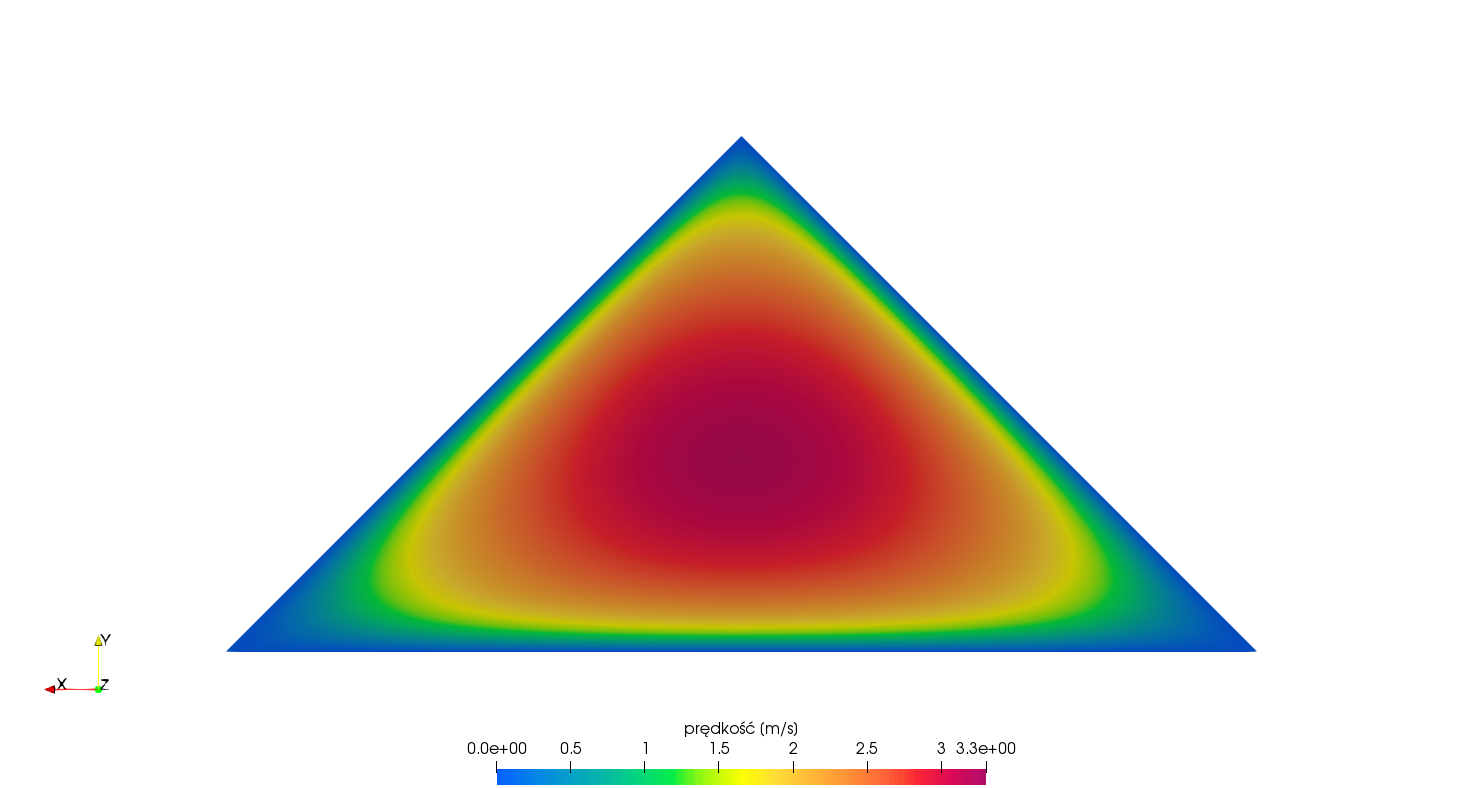
\includegraphics[width=.28\textwidth]{case_02_middle_plane_velocity}}\hfill
  \subfloat[][]{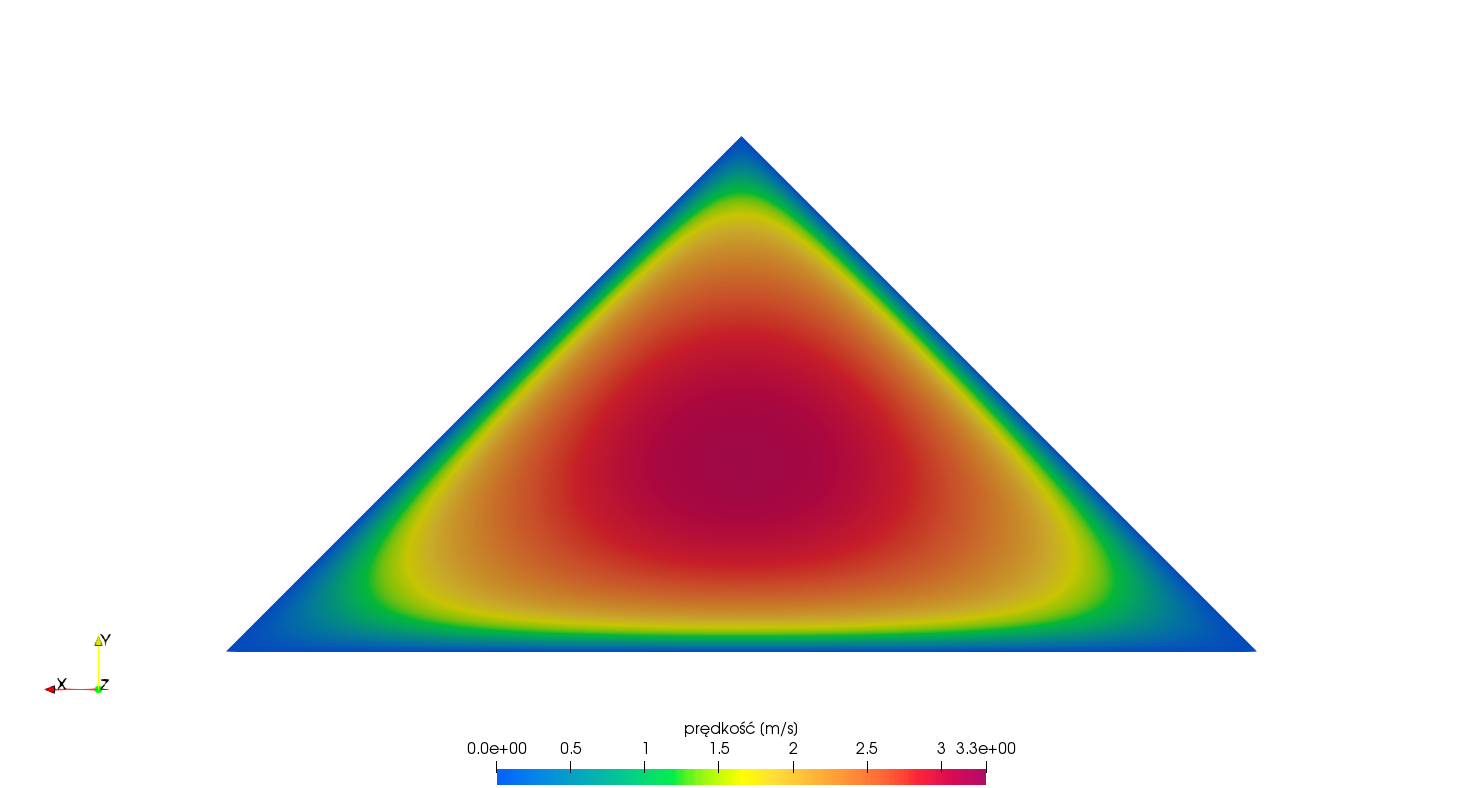
\includegraphics[width=.28\textwidth]{case_02_outlet_velocity}}\par
  \raisebox{5pt}{\parbox[b]{.1\textwidth}{wariant 3}}%
  \subfloat[][]{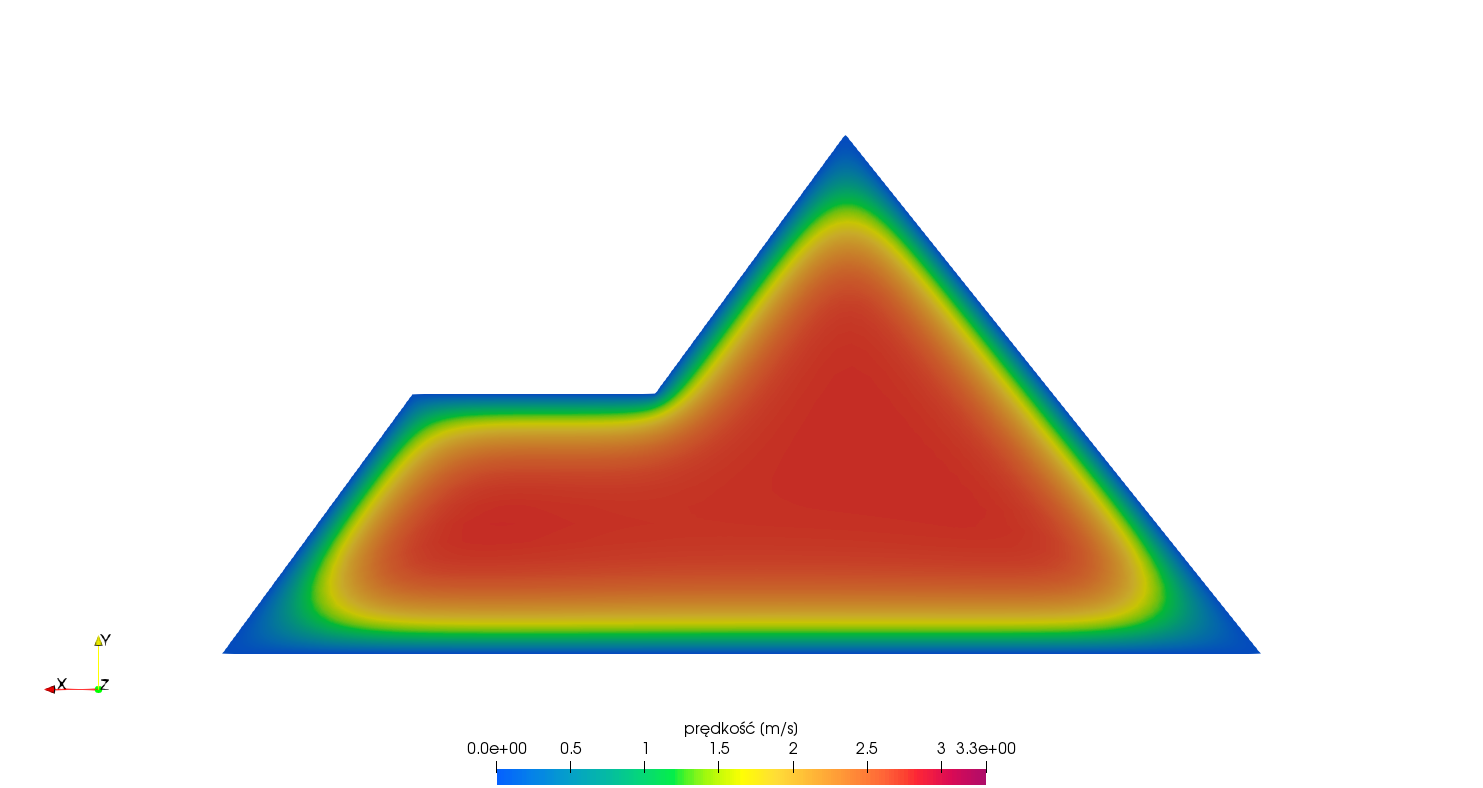
\includegraphics[width=.28\textwidth]{case_03_inlet_velocity}}\hfill
  \subfloat[][]{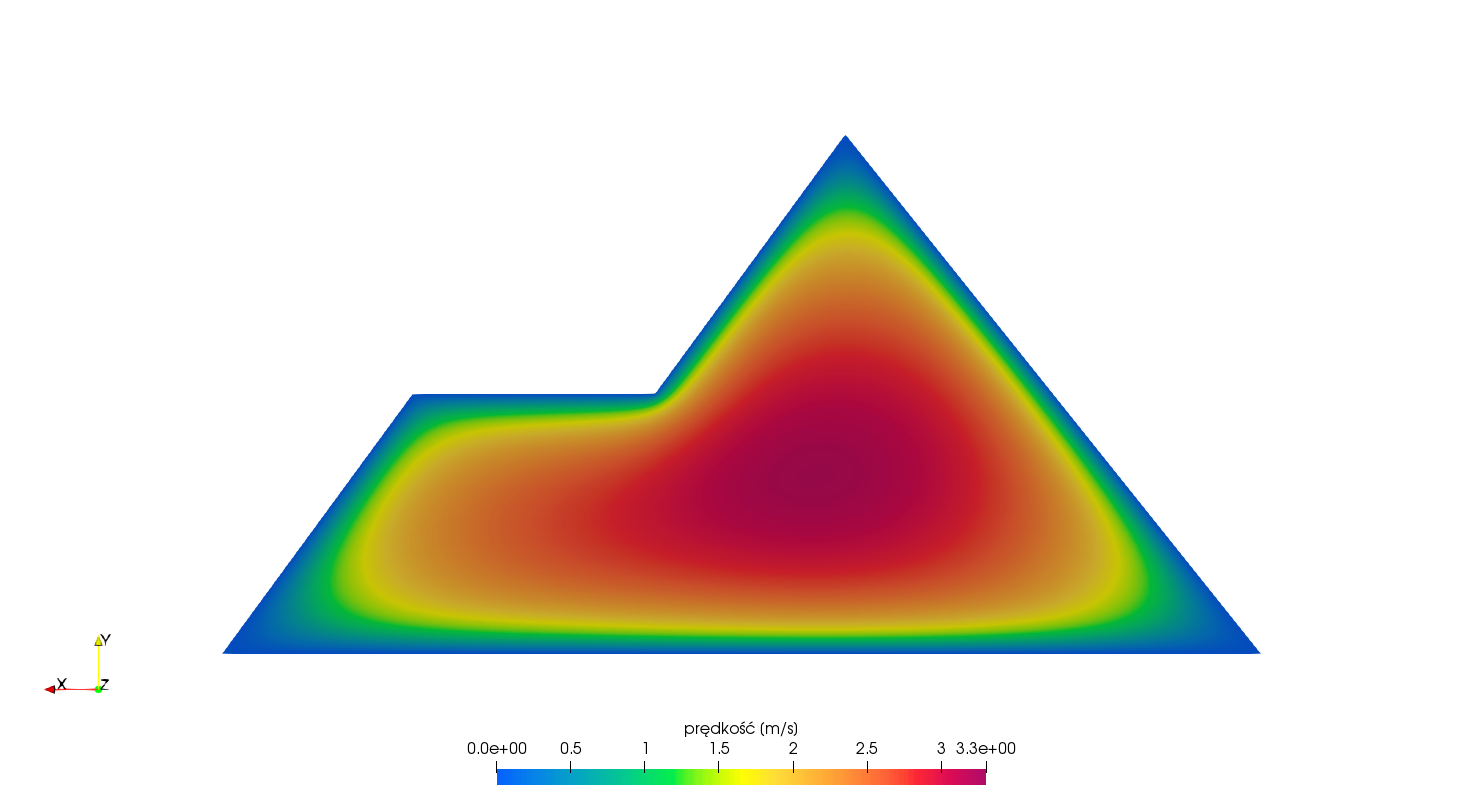
\includegraphics[width=.28\textwidth]{case_03_middle_plane_velocity}}\hfill
  \subfloat[][]{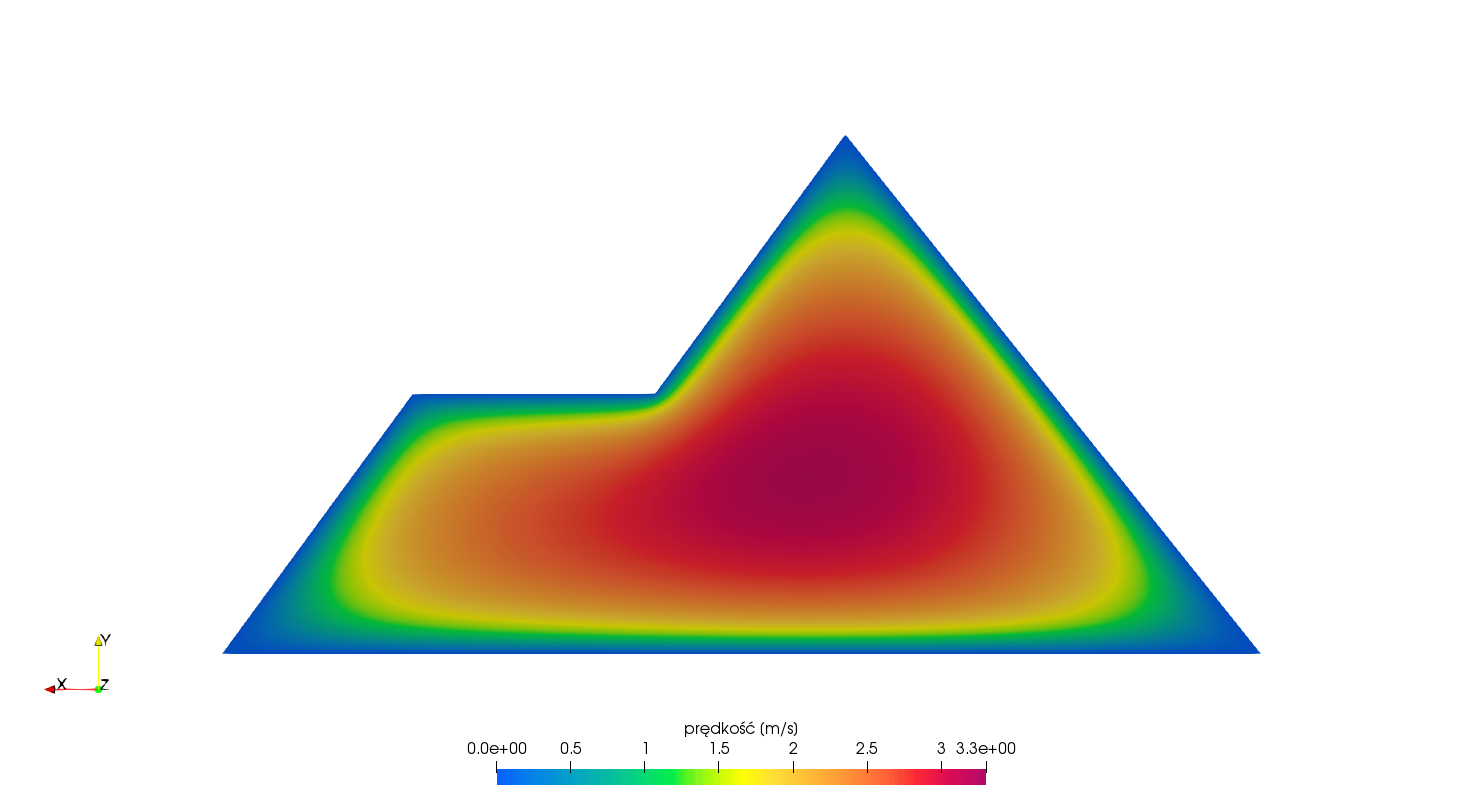
\includegraphics[width=.28\textwidth]{case_03_outlet_velocity}}
  \caption{Fields}
  \label{abc}
\end{figure*}



\subsection{Ocena nierównomierności rozkładu prędkości}





\subsection{Rozkład energii kinetycznej turbulencji}
Napisać co to ta energia kienetyczna turb.

\begin{figure*}
  \centering
  \raisebox{5pt}{\parbox[b]{.1\textwidth}{wariant 1}}%
  \subfloat[][]{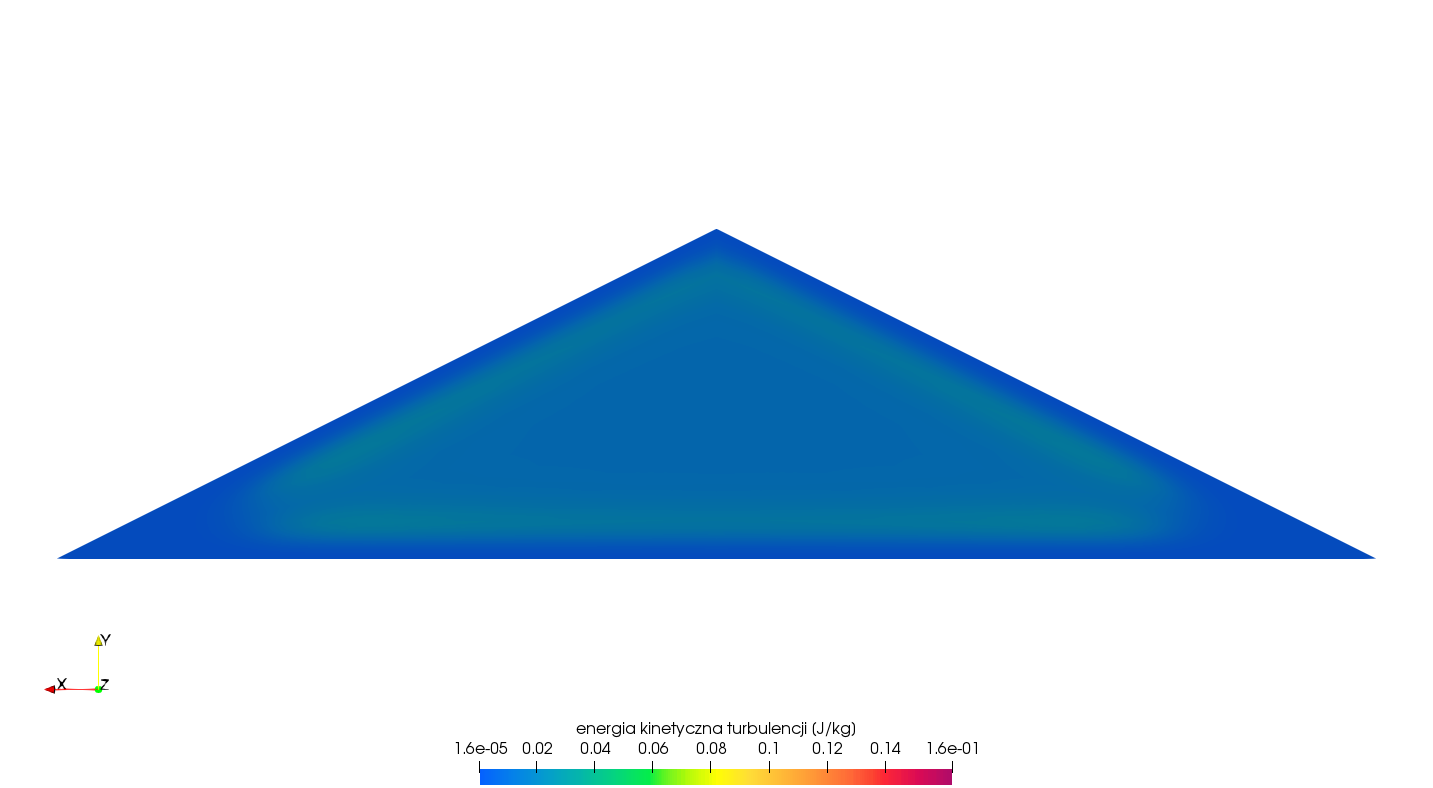
\includegraphics[width=.28\textwidth]{case_01_inlet_turb_k}}\hfill
  \subfloat[][]{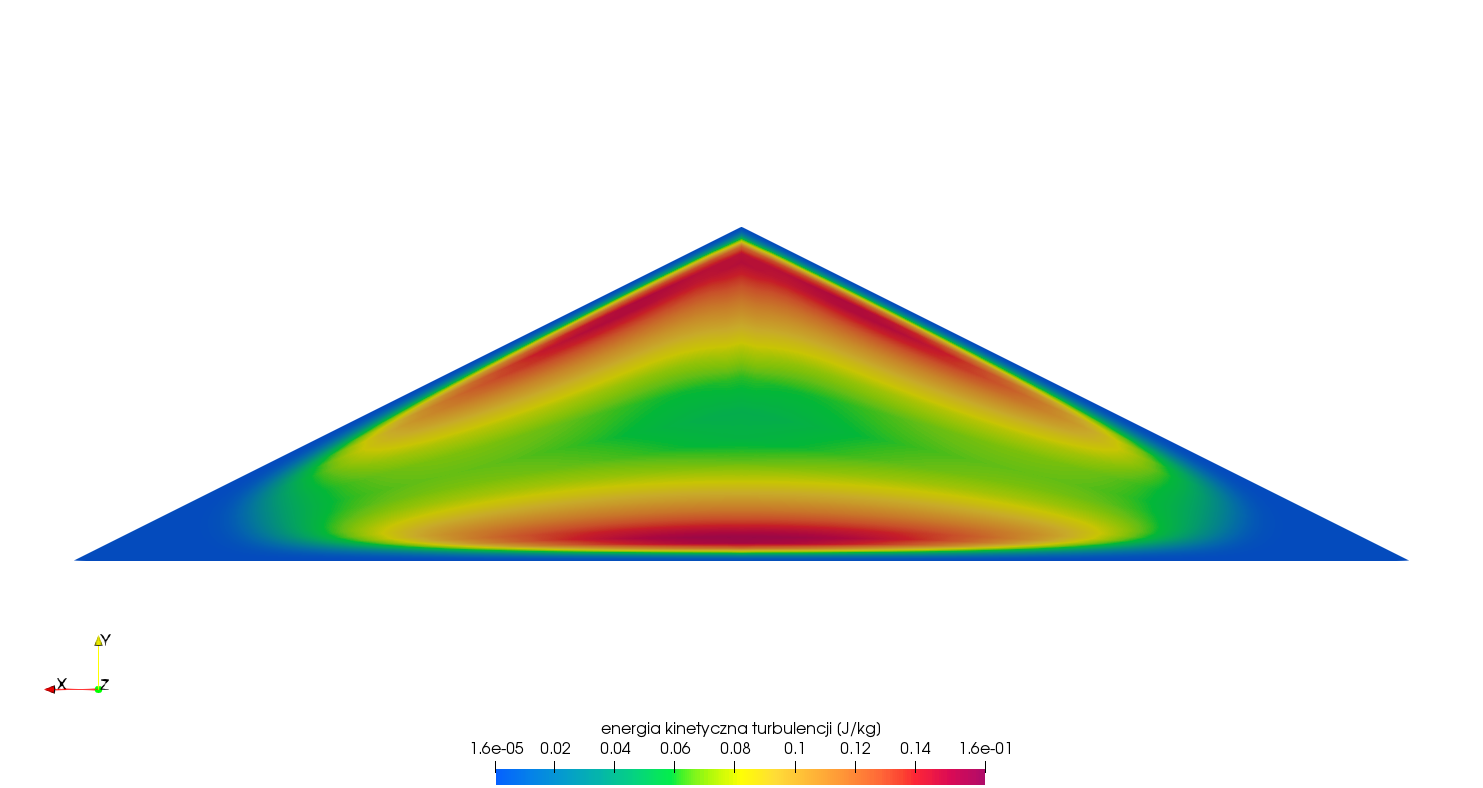
\includegraphics[width=.28\textwidth]{case_01_middle_plane_turb_k}}\hfill
  \subfloat[][]{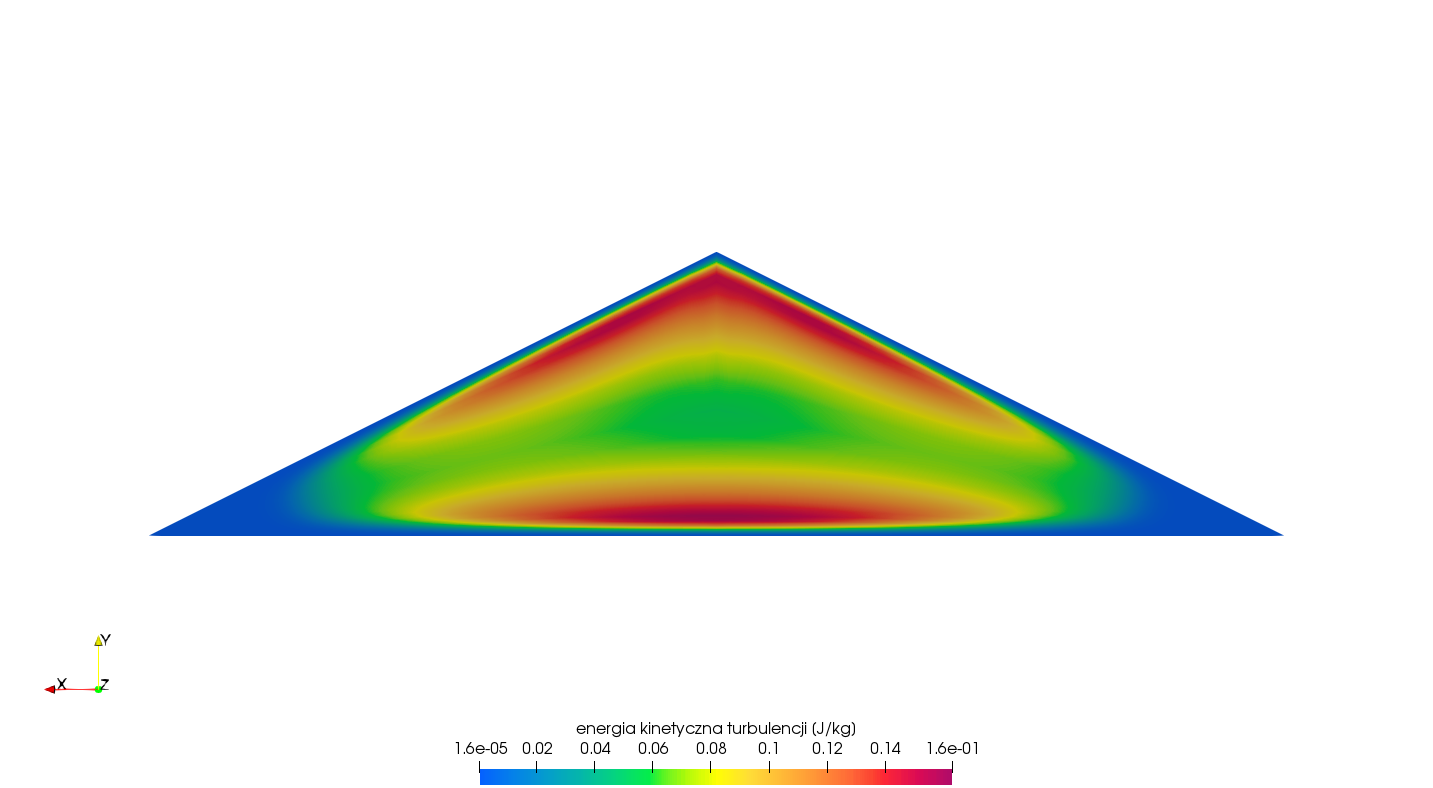
\includegraphics[width=.28\textwidth]{case_01_outlet_turb_k}}\par
  \raisebox{5pt}{\parbox[b]{.1\textwidth}{wariant 2}}%
  \subfloat[][]{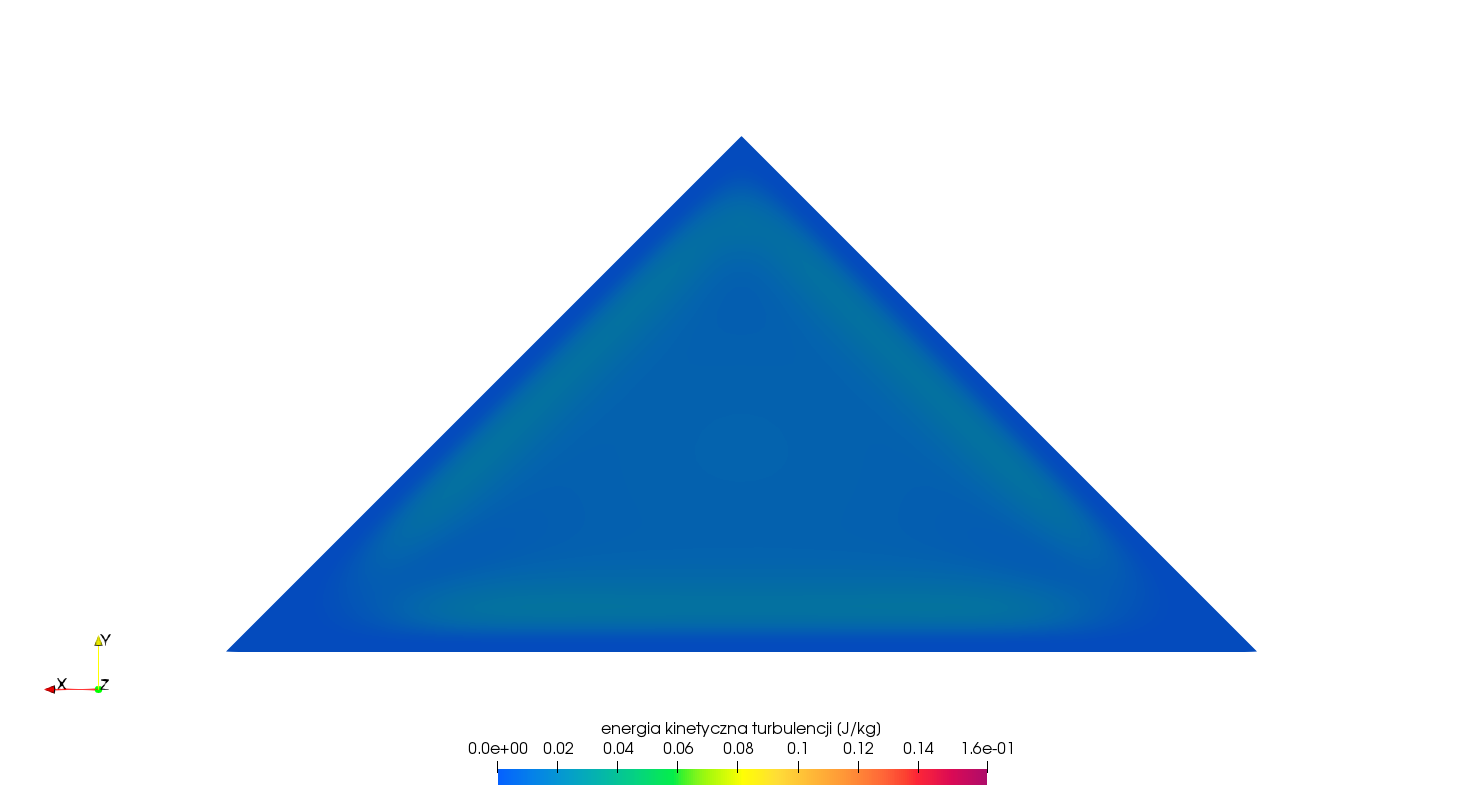
\includegraphics[width=.28\textwidth]{case_02_inlet_turb_k}}\hfill
  \subfloat[][]{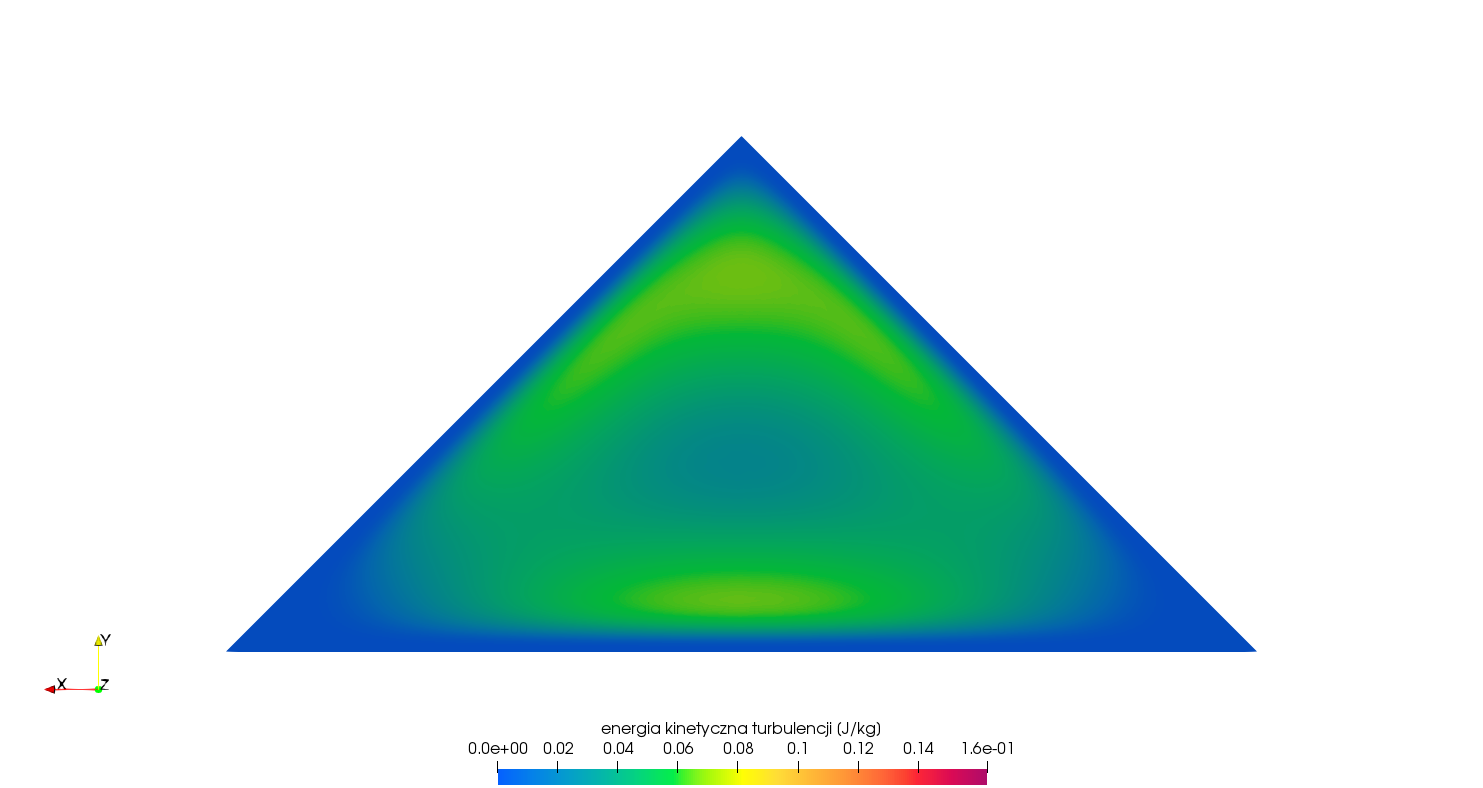
\includegraphics[width=.28\textwidth]{case_02_middle_plane_turb_k}}\hfill
  \subfloat[][]{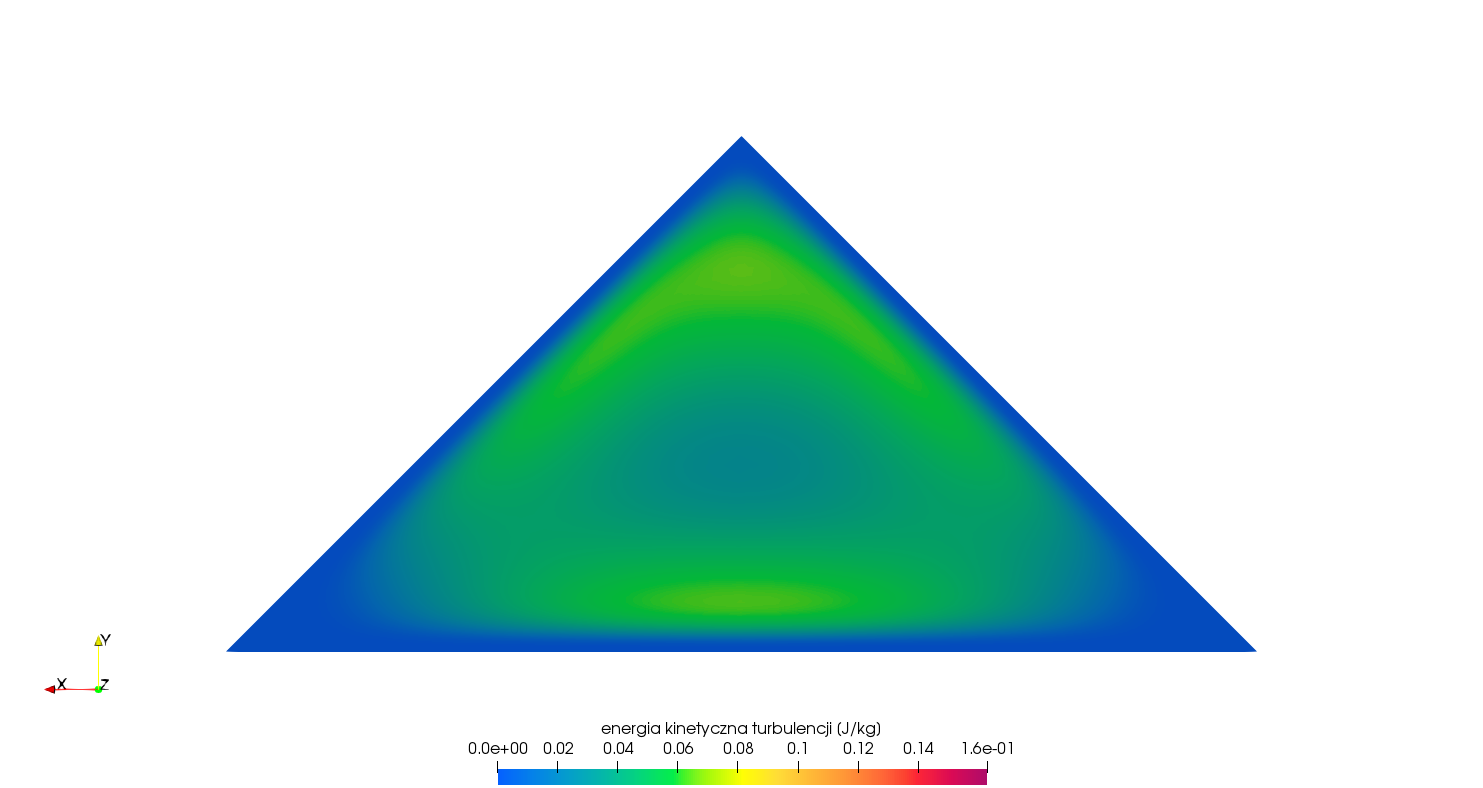
\includegraphics[width=.28\textwidth]{case_02_outlet_turb_k}}\par
  \raisebox{5pt}{\parbox[b]{.1\textwidth}{wariant 3}}%
  \subfloat[][]{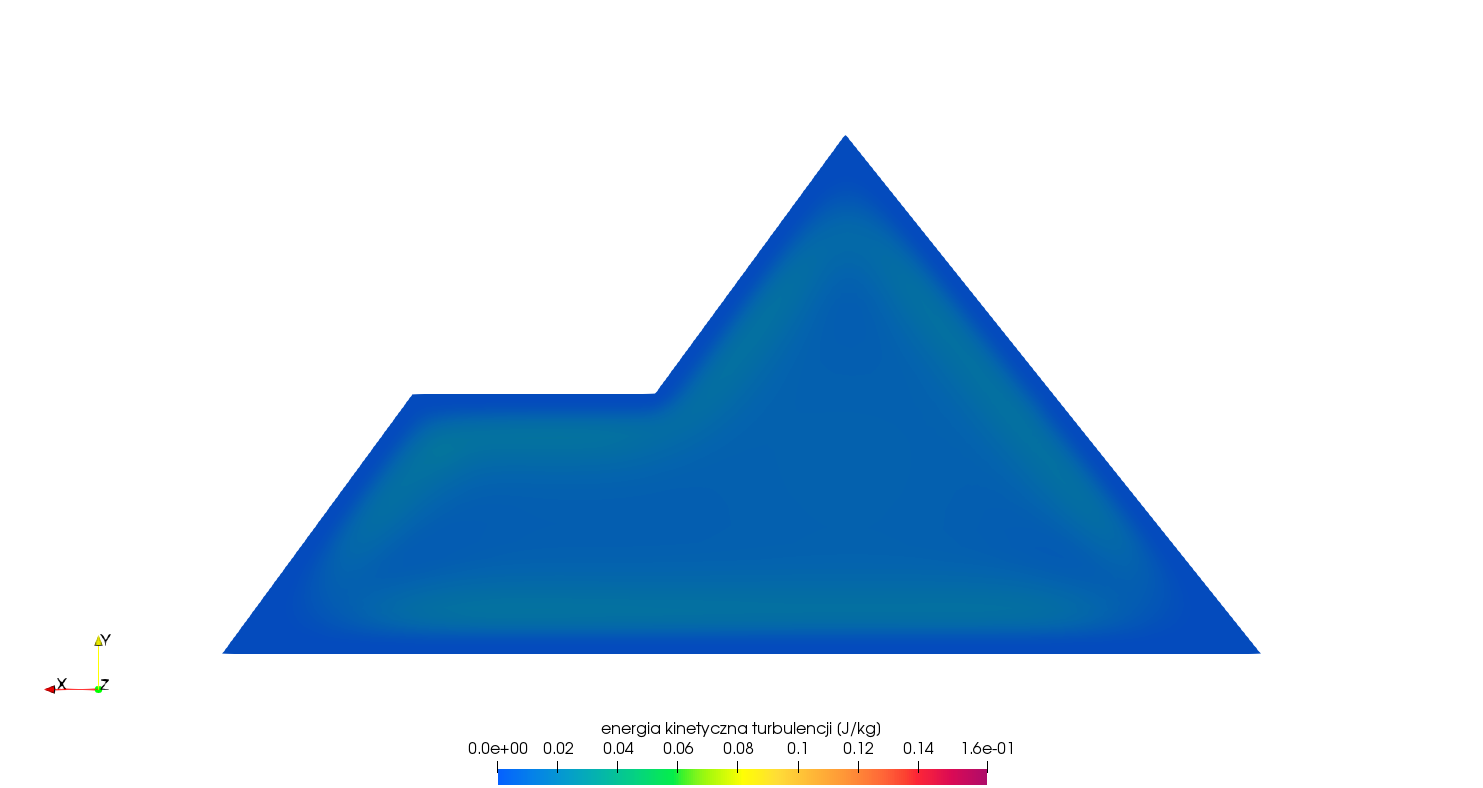
\includegraphics[width=.28\textwidth]{case_03_inlet_turb_k}}\hfill
  \subfloat[][]{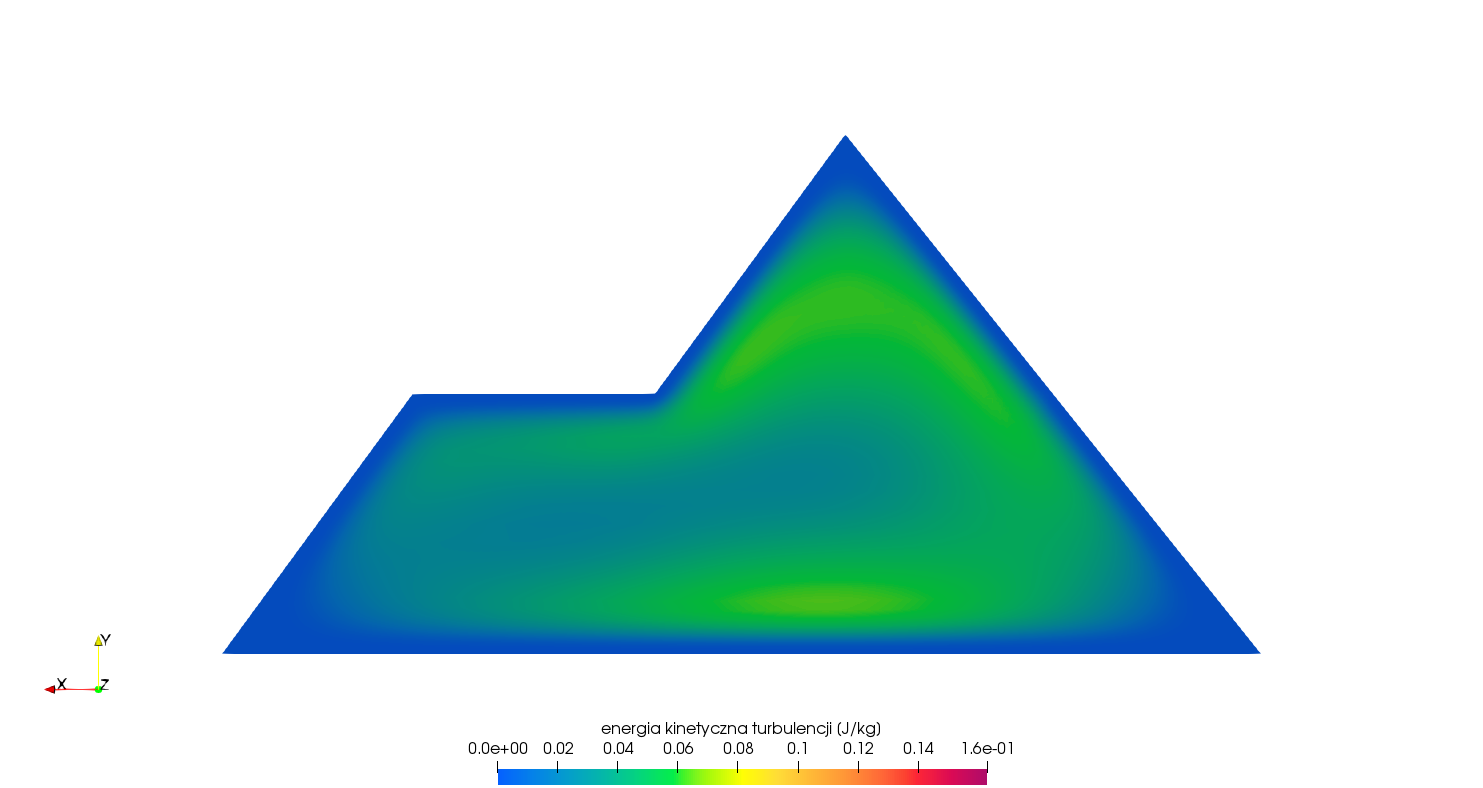
\includegraphics[width=.28\textwidth]{case_03_middle_plane_turb_k}}\hfill
  \subfloat[][]{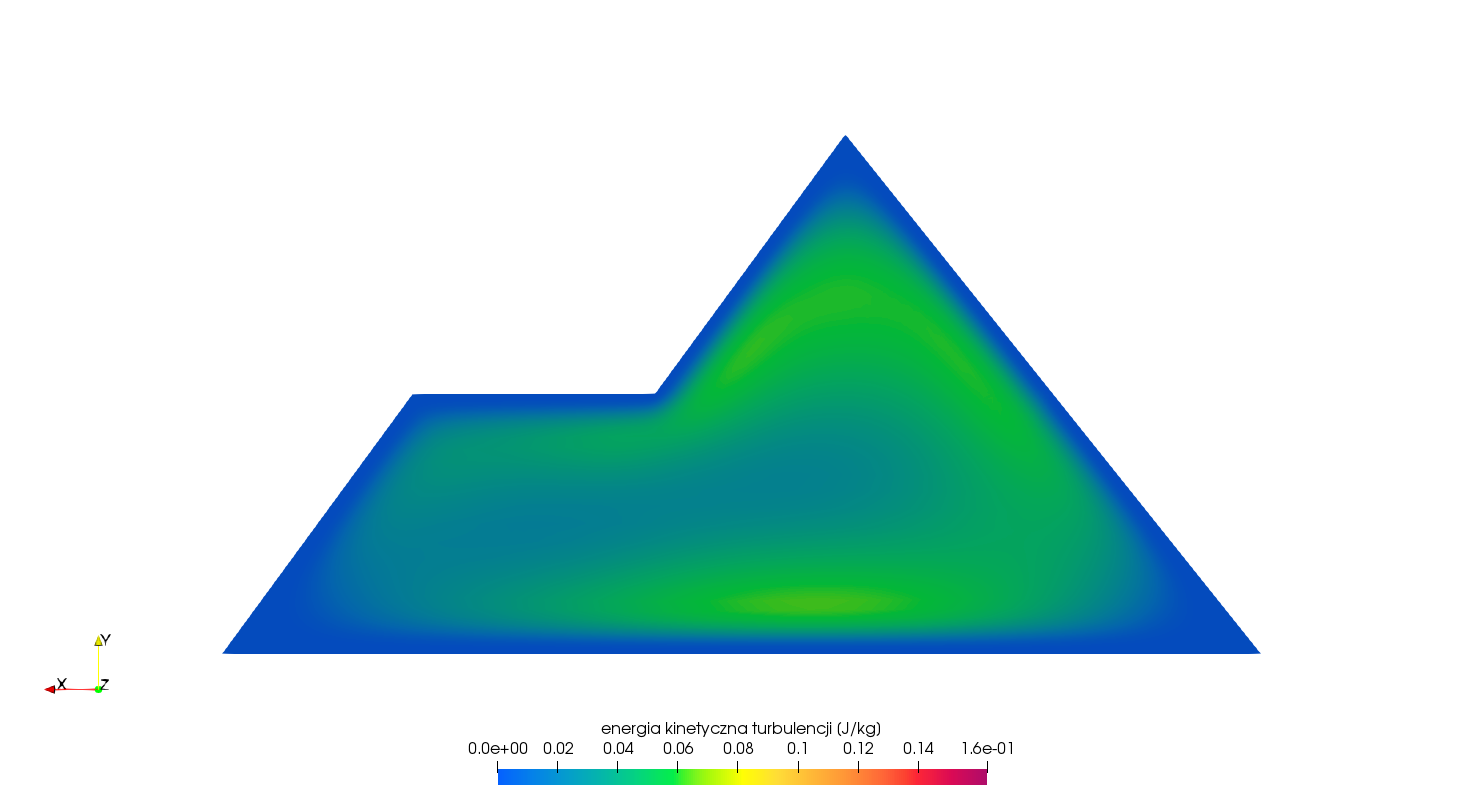
\includegraphics[width=.28\textwidth]{case_03_outlet_turb_k}}
  \caption{Fields}
  \label{subplots1310}
\end{figure*}



\subsection{Współczynnik strat ciśnienia}

Obliczenia zostały wykonane przy następujących założeniach:
\begin{itemize}
\item średnia prędkość w kanale: 2 m/s
\item gęstość płynu: 1 kg/m$^3$
\item długość przekładki: 1,1 m
\end{itemize}

//wzory tutaj napisać??

\begin{table}[]
\begin{tabular}{|l|l|l|l|}
\hline
 & wariant 1 & wariant 2 & wariant 3 \\ \hline
całkowita strata ciśnienia w kanale {[}Pa{]} & 16.73 & 13.62 & 14.73 \\ \hline
strata ciśnienia w przeliczeniu na metr długości {[}Pa/m{]} & 15.21 & 12.38 & 13.39 \\ \hline
współczynnik strat ciśnienia {[}-{]} & 6.08 & 4.95 & 5.36 \\ \hline
\end{tabular}
\end{table}

\subsection{Analiza naprężeń na dolnej ściance}

Opisać w którym miejscu i jak wyznaczono rozkład tych naprężeń. I o czym mówią te naprężenia. 

\begin{figure}[!h]
\centering
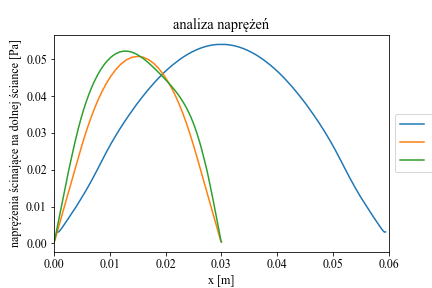
\includegraphics[width=0.8\columnwidth]{wall_shear} 
\caption{Simulation Results}
\label{fig_sim}
\end{figure} 

\section{Interpretacja wyników i wnioski}

ogólnie 1 najlepszy, potem porównać 2 i 3 który lepszy (2 najlepszy w wykonaniu), porównanie w formie tabeli??

\section{Propozycja poszerzenia badań}

\begin{itemize}
\item analiza przepływu przy zablokowanym wylocie (dosunięcia przekładek do ściany)
\item wykonanie nowego wariantu geometrycznego polegjącego na umieszczeniu otworów między poszczególymi przekładkami
\item analiza przepływu powietrza w całej komorze
\end{itemize} 


%\appendices
%\section{What Goes in the Appendices} \label{App:WhatGoes}
%The appendix is for material that readers only need to know if they are studying the report in depth. Relevant charts, big tables of data, large maps, graphs, etc. that were part of the research, but would distract the flow of the report should be given in the Appendices. 
%\section{Formatting the Appendices} \label{App:Formatting}
%Each appendix needs to be given a letter (A, B, C, etc.) and a title. \LaTeX will do the lettering automatically.


\begin{thebibliography}{1}
% Here are a few examples of different citations 
% Book
\bibitem{kopka_1999} % Note the label in the curly brackets. Use the cite the source; e.g., \cite{kopka_latex}
H.~Kopka and P.~W. Daly, \emph{A Guide to \LaTeX}, 3rd~ed.\hskip 1em plus
  0.5em minus 0.4em\relax Harlow, England: Addison-Wesley, 1999.
\bibitem{horowitz_2005}D.~Horowitz, \emph{End of Time}. New York, NY, USA: Encounter Books, 2005. [E-book] Available: ebrary, \url{http://site.ebrary.com/lib/sait/Doc?id=10080005}. Accessed on: Oct. 8, 2008.
% Article from database
\bibitem{castlevecchi_2008}D.~Castelvecchi, ``Nanoparticles Conspire with Free Radicals'' \emph{Science News}, vol.174, no. 6, p. 9, September 13, 2008. [Full Text]. Available: Proquest, \url{http://proquest.umi.com/pqdweb?index=52&did=1557231641&SrchMode=1&sid=3&Fmt=3&VInst=PROD&VType=PQD&RQT=309&VName=PQD&TS=1229451226&clientId=533}. Accessed on: Aug.~3, 2014.
% Conference Paper from the Internet
\bibitem{lach_2010}J.~Lach, ``SBFS: Steganography based file system,'' in \emph{Proceedings of the 2008 1st International Conference on Information Technology, IT 2008, 19-21 May 2008, Gdansk, Poland.} Available: IEEE Xplore, \url{http://www.ieee.org}. [Accessed: 10 Sept. 2010].
% Web page, no author
\bibitem{a_laymans_explanation}``A `layman's' explanation of Ultra Narrow Band technology,'' Oct.~3, 2003. [Online]. Available: \url{http://www.vmsk.org/Layman.pdf}. [Accessed: Dec.~3, 2003]. 
\end{thebibliography}

% This is a hand-made bibliography. If you want to use a BibTeX file, you're on your own ;-)














\end{document}
